% !TeX spellcheck = en_US
\chapter{DevOps}

DevOps is a set of practices to build, test and release your code / software in small increments (source \href{https://youtu.be/j5Zsa_eOXeY}{freeCodeCamp.org})

\begin{itemize}
	\item The name comes from the name of two teams: Development team and Operations team.
	\begin{itemize}
		\item Development team creates the plan, designs and builds the software
		\item Operation team tests and feedback on the implementation
	\end{itemize}
	\item DevOps' approach aim to improve efficiency, deliver and deploy more quickly
	\item Steps of DevOps:
	\begin{itemize}
		\item Plan: work with your team to decide on the specifications for some features
		\item Code
		\item Build: make releases for different OSs
		\item Test: automatic (/ac{aka} continuous integration), manual testing (\ac{aka} quality assurance)
		\item Release: deliver your software in a way that users won't know if there are any problems. Perhaps show to a subset of users to check for issues
		\item Deploy
		\item Operate: scaling, ensure enough servers, \etc
		\item Monitor
	\end{itemize}
\end{itemize}

\begin{figure}[hbt!]
	\centering
	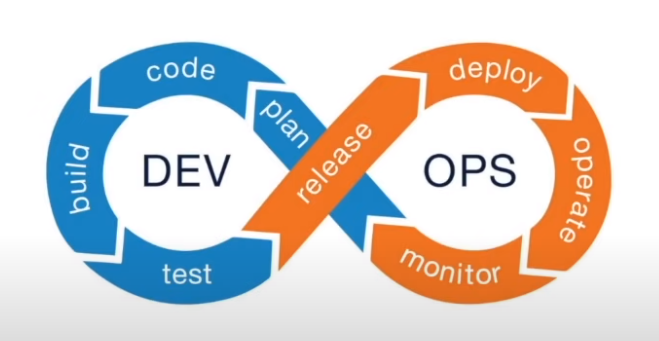
\includegraphics[width=0.7\textwidth]{DevOps.png}
	\caption{Steps of DevOps \href{https://youtu.be/j5Zsa_eOXeY}{freeCodeCamp.org}}
\end{figure}

\section{DevOps Engineering Pillars}
\begin{itemize}
	\item DevOps Engineering is about being able to automate build, test, release and monitor applications
	\item Pull request automation: help developers build thing faster
	\begin{itemize}
		\item Share code changes using \texttt{git} tools
		\item Dealing with pull request, merge request
		\item Feedback on pull request: code style, architecture, scaling
	\end{itemize}
	\item Deployment automation: help you deploying your code in a way that users don't complain
	\item Application performance management: automation around making sure everything is healthy, detecting downtime, rolling back if there is problem.
\end{itemize}

You can automate:
\begin{itemize}
	\item Test run (\ac{CI}) for each proposed changes
	\item Security scanning
	\item Notifications to reviewers, the right people to review at the same time
	\item Help developer to change proposals, get review and merged within 23 hours
\end{itemize}

\subsection{Application Performance Management}
\begin{itemize}
	\item Metrics: numeric measurements of KPIs
	\item Logging: text descriptions of what is happening during processing
	\item Monitoring: take metrics and logs to convert them into health metrics
	\item Alerting: of monitoring detects of problem, it notifies developers
\end{itemize}

\section{Testing and Test Driven Development}
\begin{itemize}
	\item \ac{TDD} is a coding methodology where the tests are written before the code is written
	\item Test levels derived from factory production:
	\begin{itemize}
		\item Unit test
		\item Integration test: ensure a few components work together
		\item System / end to end tests: ensure the whole product works
		\item Acceptance test: after being launched, are the customers' needs are satisfied
	\end{itemize}
	\item Testing is about knowing when something breaks and where
\end{itemize}

\section{Continuous Integration}
\begin{itemize}
	\item \ac{CI} is the practice for the developers to commit the changes to shared repositories, trigger a workflow on a CI server
\end{itemize}